\section{Theoretical background}
\subsection{Engineering design process}

The creation of a physical product destined to be used by people, requires a methodical approach. In product design, the steps involved in the creative process can be summarised by the engineering design process. To build a product with a specified performance goal, the engineering design process is a plan that involves a number of steps, where certain parts may need to be repeated many times before production of a final product can begin. Figure \ref{fig:eng-design-process} depicts the general work-flow \cite{nasa}.

\begin{figure}[h]
\begin{center}
\makebox[\textwidth][c]{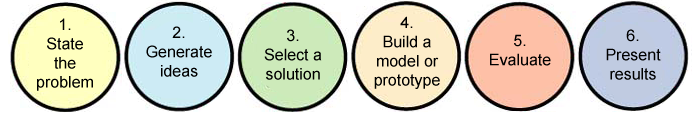
\includegraphics[width=1\textwidth]{figures/design-process-4.png}}
\caption{\small {\it {Steps in the engineering design process}}} \label{fig:eng-design-process}
\end{center}
\end{figure}

The first step requires defining the problem, why it is important to solve, and the resulting design requirements will state the important characteristics that the solution must meet to succeed. A way to identify the requirements, is to analyse a similar, existing product, in this case Houben et. al's prototype. \\

\subsection{Brainstorming}

The second step requires using methods for choosing a possible solution. Brainstorming can help in this matter, and consists of gathering solution ideas, without criticism from other people. Popularised by Alex F. Osborn in 1948, it is designed to maximize the productivity of groups engaged in idea generation \cite{osborn1948your}. \\

The ideas are then discussed in the third step. A look is taken at whether each possible solution meets the design requirements, and the solutions that do not meet the requirements are rejected \cite{wikiBrainstorm}. \\

\subsection{Prototyping}
\label{section-prototyping}

The fourth step is the prototyping process. In product design, a prototype is a tangible artefact that is used by both the designers and the users to help the designers selecting the best solution. A successful prototype has many positive characteristics: it supports creativity by uncovering relevant information from the users. It encourages communication between designers and users. Finally, it permits early evaluation through methods such as usability studies and informal user feedback. \\

Beaudouin-Lafon et. al. (2003) describe prototypes as being characterised by four dimensions, namely, their representation, precision, interactivity, and evolution \cite{Beaudouin-Lafon}. \\

The \emph{representation} of a prototype is its form, such as a paper sketch or a 3D printed model. A rough sketch on paper or a virtual CAD model can constitute a prototype, and are called offline and online prototypes, respectively. Offline prototypes are inexpensive and quick, which permits a rapid iteration cycle. \\

The \emph{precision} of a prototype refers to the level of detail at which the prototype is to be evaluated. Terms like low-fidelity and high-fidelity are often used in the literature. High detail is generally not necessary, as some refinement to the design is to be expected. Prototypes are often built using very limited engineering detail as compared to final production intent. \\

The \emph{interactivity} describes the extent to which the user can actually interact with the prototype. It could be watch-only or fully interactive. The interactivity levels can be categorized in fixed, fixed-path, and open prototypes: a fixed prototype \emph{illustrates} what the experience might look like, e.g. a paper prototype. A fixed-path prototype provides the \emph{experience} of what the interaction might be like, and lastly, an open prototype allows to \emph{test} the interaction with the users. \\

The \emph{evolution} describes the expected life cycle of the prototype (e.g., throw away or iterative). Prototypes have different life spans. \emph{Evolutionary} prototypes are not thrown away, and will be part of the final system. \emph{Iterative} prototypes evolve to change some details, such as increasing precision. Finally, \emph{rapid} prototypes have a very short life-span, and are created in order to be evaluated before being thrown away.

\subsection{Rapid prototyping}

Offline prototyping techniques can have varying degrees of complexity, such as a simple paper and pencil sketch to a 3D printed model. The fastest form of prototyping involves paper, but its precision is not at the level of a tangible 3D model. Up until the emergence of virtual prototyping with CAD applications, prototyping was manual, and tended to be craft-based, thus very slow \cite{chua2010}. In the 1980s, virtual prototyping became more widespread, as computer tools became more mature. Virtual models could now be analysed and modified as if they were physical prototypes, and several iterations of designs could be easily carried out. But as the prototypes became more complex, the time required to make a physical model increased, and therefore craft-based production of a physical prototype became tedious \cite{chua2010}. \\

A new type of prototyping has therefore emerged in the 1980s, called rapid prototyping (RP). Rapid Prototyping can be defined as techniques used to quickly fabricate a scale model of a part or assembly, using three-dimensional computer aided design (CAD). \\

Rapid Prototyping has also been referred to as solid free-form manufacturing, computer automated manufacturing, and layered manufacturing \cite{efunda}. An RP model's most used scenario is for testing various qualities of a physical product, and in some cases, the RP part can be the final part, but typically the RP material is not strong or accurate enough. \\

There exists many experimental RP techniques such as Stereolithography (SLA), Digital Light Processing (DLP), Laminated Object Manufacturing (LOM), Electron Beam Freeform Fabrication (EBF3), Fused Deposition Modelling (FDM), and more \cite{wiki3D}. The latter was specifically used in this project, because of its almost ubiquitous presence in universities, fab-labs, and hackerspaces. \\

The main reasons for using Rapid Prototyping are very compelling. It decreases costly mistakes and engineering changes, thus minimizing development time. By being able to have a look at the product early in the design process, mistakes can be corrected, and changes can be made while they are still inexpensive. \\

Rapid prototyping of physical parts can be performed in many different ways, but they all adopt the same basic methodology \cite{chua2010-p10}:

\begin{itemize} \itemsep0em
  \item A virtual model is designed in a CAD application.  It represents the part that is physically built as an enclosed volume, and will specify the inside, the outside, and boundaries of the model.
  \item The model to be built is next converted into an STL (Stereo Lithography) file format. The STL format approximates the surfaces of the model by polygons.
  \item A program analyses the STL file, and ``slices'' the model into cross-sections. It generates paths to be filled and calculates the amount of material to be extruded, in the case of a 3D printer that uses fused deposition modelling \cite{slic3r}. In short, it converts a digital 3D model into printing instructions for a 3D printer.
  \item The model and any supports are removed. The surface of the model is then finished and cleaned for imperfections \cite{efunda}.
\end{itemize}

\subsection{User-centered design}

As Human–computer interaction (HCI) involves the design of interaction between users and computers, elements of HCI can be applied to the design process of the device presented in this project. HCI is user-centered and iterative (Norman \& Draper, 1986) \cite{Norman-1986}, and those two characteristics fit well within the design process of this project, as they allow for requirements, usability problems, and performance issues to be identified early, and improved at each iteration. The latter involves therefore multiple loops through the steps of design, implementation, and test, represented in steps 3 to 5 on figure \ref{fig:eng-design-process}. \\

User-centered design is a problem solving process that requires analysing how users are likely to use a product, and to test the validity of assumptions with regard to user behaviour. Such testing is necessary as it is difficult to predict a first-time user's learning curve, and what they might experience.

\subsection{Evaluation}
\label{section-evaluation}

This leads to the fifth step in figure 1 -- user-centered design implies choosing evaluation methods for usability testing. As Jakob Nielsen describes in the book Usability Engineering (1993) \cite{jakob-1993}, there are a couple of simple and cheap methods available, i.e. the use of scenarios, thinking-aloud, and heuristic evaluation. The latter is more adapted to user-interface design, but the thinking-aloud method can be applied to evaluating a physical product, and is considered to be cheap, robust, flexible, and easy to learn \cite{jakob-1993}. \\

Thinking-aloud consists in having a user perform a set of tasks with the prototype under evaluation. The user is then asked to ``think out loud'' while using the prototype. This allows an observer to determine what the user is doing, and why. This insight can then be used to pinpoint elements of the prototype that are impractical, misunderstood, etc., as it involves getting a user to verbalize their thought processes. The observer can videotape, or take notes for later analysis. \\

The minimum number of users for performing a qualitative evaluation, has also been shown to be quite low. In the article ``Usability engineering at a discount'' (1989) \cite{Nielsen-1989}, Jakob Nielsen argues that five users is just enough to acquire useful data, where the first round of testing can gather 85\% of the usability problems. ``Discount usability'' often gives better results than ``deluxe usability'' because its methods drive an emphasis on early and rapid iteration with frequent usability input \cite{nielsen-discount}.